\documentclass[twoside,11pt,preprint]{article}
\usepackage{tikz}
\usetikzlibrary{positioning, shapes.geometric, arrows.meta, fit}
\usepackage{pgfplots}
\pgfplotsset{compat=1.18}
\usepackage{amsmath}

\begin{document}

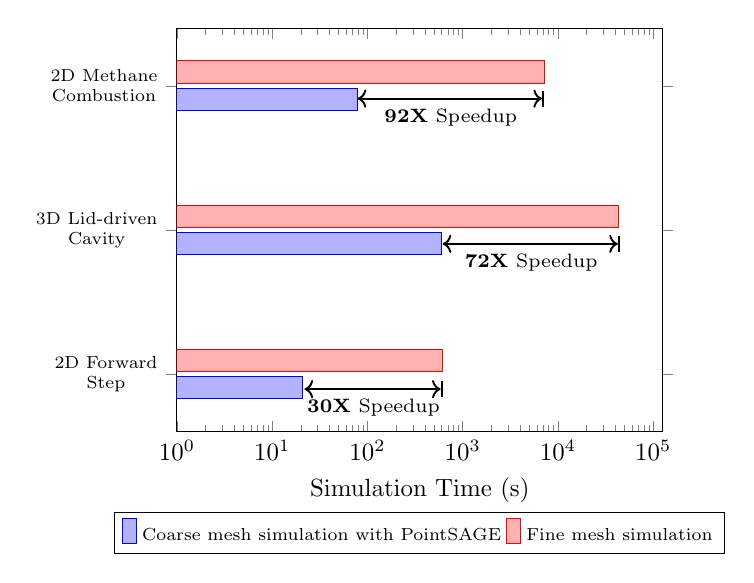
\begin{tikzpicture}[scale=0.9] % Adjust the scale factor as needed
    \begin{axis}[
        xmin=1, % Set xmin to 1 to avoid log(0)
        xlabel={Simulation Time (s)}, % Set xlabel instead of ylabel for horizontal bars
        xmode=log, % Set x-axis to logarithmic scale
        ytick=data,
        yticklabels={2D Forward \\Step, 3D Lid-driven \\Cavity, 2D Methane \\Combustion},
        yticklabel style={align=center, font=\scriptsize}, % Set font size for y-axis labels and align to center
        legend style={at={(0.5,-0.2)}, anchor=north, legend columns=-1, font=\scriptsize}, % Adjust font size here
        enlarge y limits={0.2}, % Increase the distance between bars and axis
        xbar,
        bar width=9pt,
        legend image code/.code={
            \draw [#1] (0cm,-0.1cm) rectangle (0.2cm,0.25cm); },
        ]
        \addplot coordinates {(21,0) (600,1) (78,2)};
        \addplot coordinates {(610,0) (43200,1) (7146.67,2)};
        \legend{Coarse mesh simulation with PointSAGE, Fine mesh simulation}
    \end{axis}
    % Calculate and add arrows with annotations
    \draw[<->|, line width=0.7pt] (1.8,0.6) -- (3.75,0.6) node[midway,below, font=\scriptsize] {\textbf{30X} Speedup};
    \draw[<->|, line width=0.7pt] (3.75,2.65) -- (6.25,2.65) node[midway,below, font=\scriptsize] {\textbf{72X} Speedup};
    \draw[<->|, line width=0.7pt] (2.55,4.7) -- (5.18,4.7) node[midway,below, font=\scriptsize] {\textbf{92X} Speedup};
\end{tikzpicture}

\end{document}